\section{Equations of motion at second order}
From the full Bernoulli equation (\ref{Bernoulli_nl}), the second order approximation is 
 \begin{equation}
    \frac{\partial \phi_2}{\partial t} =
    -\frac{1}{2}\left[
    \left|\bnabla \phi_1\right|^2
    +\left(\frac{\partial \phi_1}{\partial z}\right)^2
    \right]
    -\frac{p_2}{\rho_w}-g z + C_2(t).\label{Bernoulli2}
\end{equation}
The usual combination with the surface kinematic boundary condition yields the second order wave equation,
\begin{equation}
\left(\frac{\partial ^{2}}{\partial t^{2}} +  \frac{\partial  }{\partial z} \right) \phi_2
    +g \frac{\partial \phi_2 }{\partial z}=- g \zeta_1 \frac{\partial^2 \phi_1 }{\partial z^2} + g \bnabla\phi_1 \bcdot\bnabla \zeta_1-\frac{\partial}{\partial
t} \left( \zeta_1 \frac{\partial^2 \phi_1}{\partial z \partial t}\right) -\bnabla \phi_1 \bcdot%
    \frac{\partial \bnabla \phi_1 }{\partial t}- \frac{\partial \phi_1 }{%
    \partial z}\frac{\partial ^{2}\phi_1 }{\partial t\partial z}\nonumber\\
    \quad \mathrm{on} \quad z=0 .  \label{surface_2b}
\end{equation}
The first term on the right hand side comes from the Taylor expansion of the left hand side around  $z=0$, 
and the four other terms are coming from eq. (\ref{surface comb}).




\section{Monochromatic waves at second order}
Plugging a single monochromatic wave solution with wavenumber ${\mathbf k}_0$, as given in chapter \ref{ch1b}, gives 
second order Stokes solution. For a linear amplitude $a=2 Z_{1,{\mathbf k}_0}^{+}$, we have  $\Phi _{1,{\mathbf
k}_0}^+=-\mathrm{i}a g/\left(2\sigma\right)$ and
\begin{equation}
    \phi_1=\frac{\cosh\left(k_0 z+k_0 h\right)}{\cosh\left(k_0 D\right)}
    \left(\Phi _{1,{\mathbf k}_0}^+
    \mathrm{e}^{\mathrm{i}\left(\mathbf{k}_0\bcdot{\mathbf x}-\sigma_0 t\right)}
    +\overline{\Phi}_{1,{\mathbf k}_0}^+
\mathrm{e}^{-\mathrm{i}\left(\mathbf{k}_0\bcdot{\mathbf
x}-\sigma_0 t\right)}\right),
\end{equation}

%%%%%%%%%%%%%%%%%%%%%%%%%%%%%%%%%%%%%%%%%%%%%%%%%%%%%%%%%%%%%%%%%%%%%%%%%%%%
\begin{figure}
\centerline{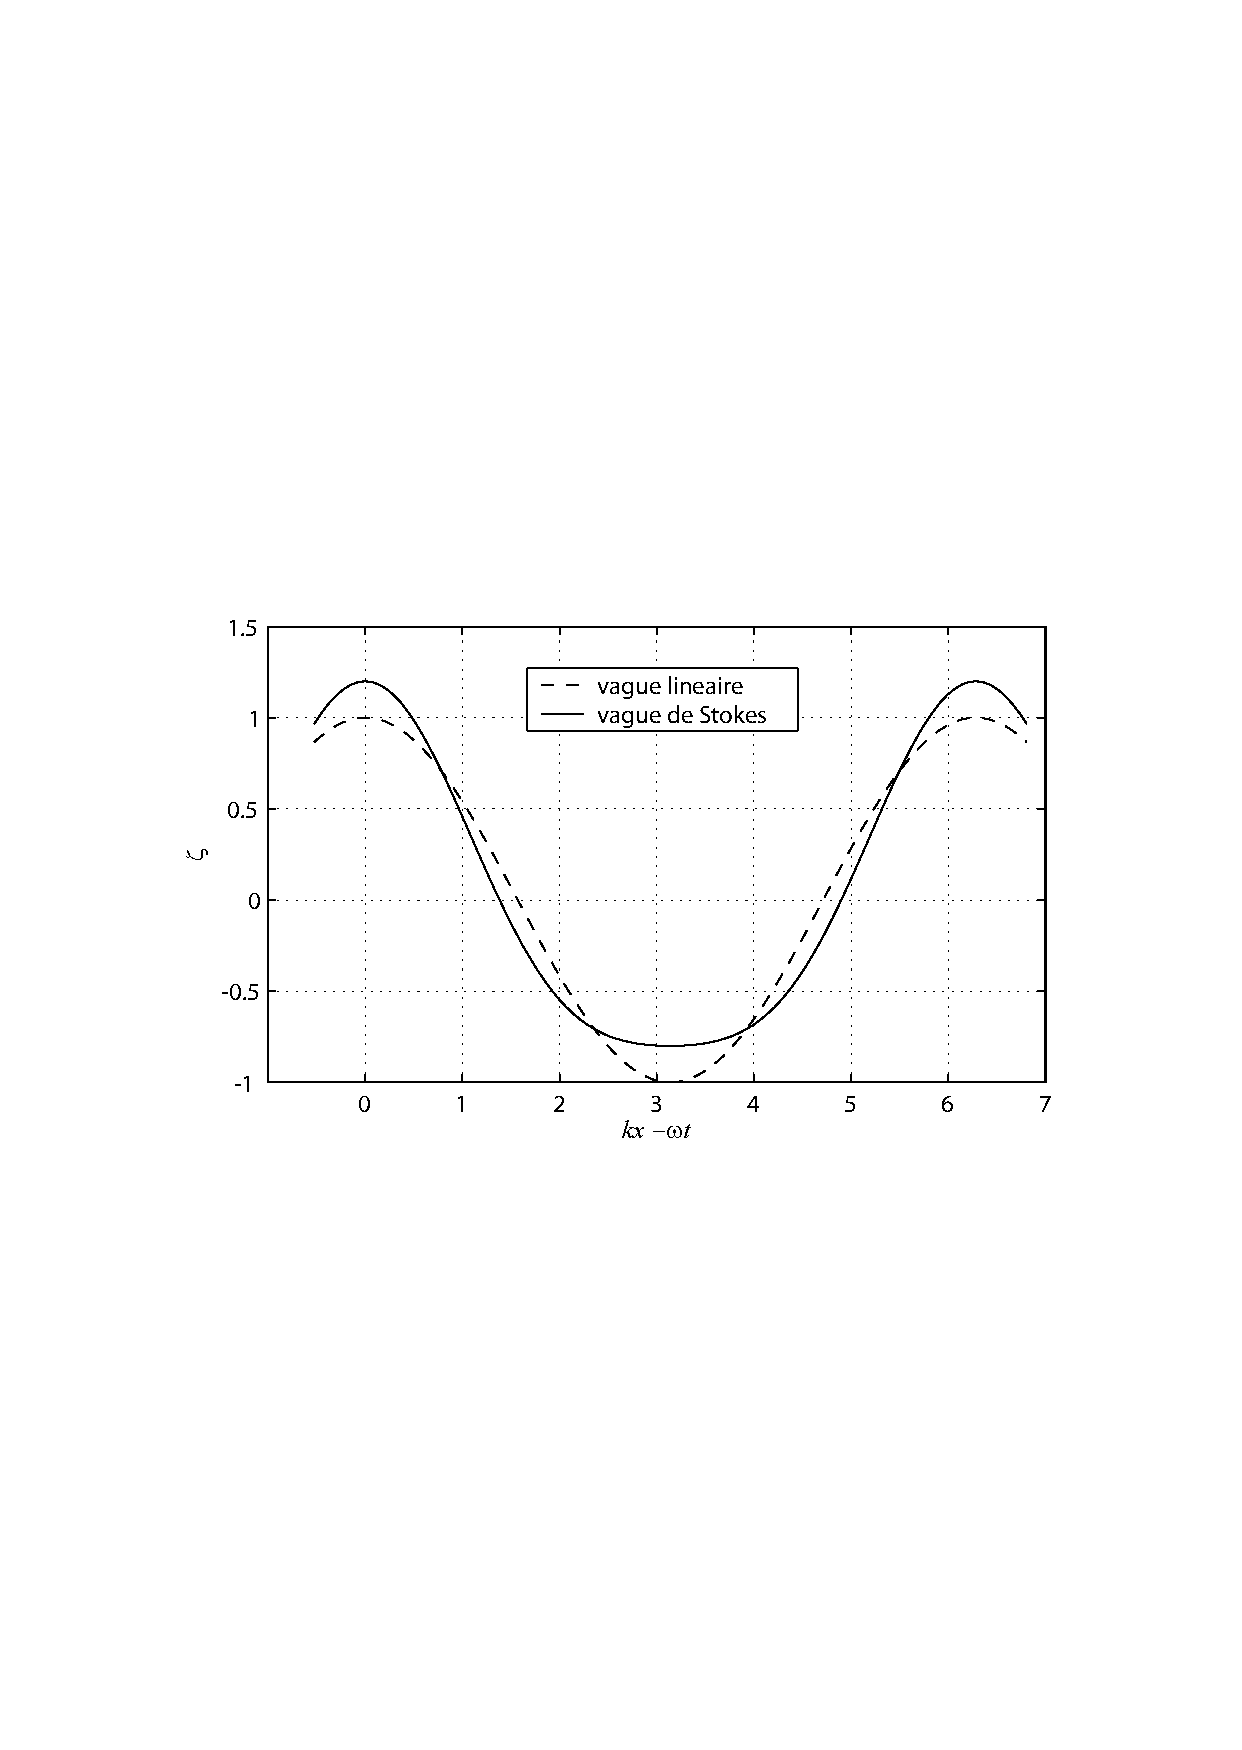
\includegraphics[width=0.6\textwidth]{FIGURES/stokes.pdf}}
%\vspace{3.64in}
\caption{Profiles of a linear Airy wave and a second order Stokes wave.} \label{stokes}
\end{figure}
%%%%%%%%%%%%%%%%%%%%%%%%%%%%%%%%%%%%%%%%%%%%%%%%%%%%%%%%%%%%%%%%%%%%%%%%%%%%
The solution is, 
\begin{equation}
    \phi_2=\frac{\cosh\left(2 k_0 z+2 k_0 h\right)}{\cosh\left(2 k_0 D\right)}
    \left(
    \Phi_{2,2 {\mathbf k}_0}^{+}
    \mathrm{e}^{\mathrm{i}\left(2 \mathbf{k}_0\bcdot{\mathbf x}-2 \sigma_0 t\right)}
    +\overline{\Phi}_{2,2 {\mathbf k}_0}^{+}
    \mathrm{e}^{-\mathrm{i}\left(2 \mathbf{k}_0\bcdot{\mathbf x}-2 \sigma_0 t\right)}
      \right)
    +2 \Phi _{2,{\mathbf 0}}^{+}
\end{equation}
avec
\begin{eqnarray}
\Phi_{2,2 {\mathbf k}_0}^{+} & = &
    D\left({\mathbf k}_0,{\mathbf k}_0\right)
        \frac{\left(\Phi_{1,{\mathbf k}_0}^{+} \right)^2}
        {\sigma^2\left(2k_0\right)-4\sigma_0^2} \\
    & =& \frac{3{\mathrm i}\sigma k\cosh\left(2kh\right)}
        {4g\sinh^3\left(kh\right) \cosh\left(kh\right)  }
        \left(\Phi_{1,{\mathbf k}_0}^{+} \right)^2,
\end{eqnarray}
and
\begin{equation}
\Phi_{2,{\mathbf 0}}^{+}  = 0,
\end{equation}
giving
\begin{equation}
    Z_{2,2{\kb}_0}^{+}
    = a^2 \frac{k\cosh\left(kh\right)\left[2+\cosh\left(2k h\right)\right]}
        {32 \sinh ^3 \left(kh\right)},
\end{equation}
and
\begin{equation}
    Z_{2,{\mathbf 0}}^{+}
    = a^2 \frac{\sigma^2}{g^2}k^2\left[\tanh^2\left(2kh\right)-1\right].
\end{equation}


The phases of the harmonics are locked with the phase of the linear waves, and the elevation and velocity 
fields are given by \citep{Dean&Dalrymple1991},
\begin{eqnarray}
    \zeta&=&a \cos \left[k\left(x- C t\right) \right)]
    + ka^2 \frac{\left[2+\cosh\left(kD\right)\right]}
        {4 \sinh^3\left(kD\right)} \cos \left[2k\left(x- C t\right) \right)]\\
    u&=&\omega a \frac{\cosh\left(kz+kD\right)}{\sinh\left(kD\right)}
        \cos \left[k\left(x- C t\right) \right)]
    + \frac{3}{4} k^2 a^2 C \frac{\cosh\left(2kz+2kD\right)}
        {\sinh^4\left(kD\right)}    \cos \left[2k\left(x- C t\right) \right)]
\end{eqnarray}
Compared to linear waves, this orbital velocity is higher the crests, and lower 
under the troughs. 




\section{Second order motion for random waves}
Before generalizing to a full wave spectrum, we note tha \cite{Miche1944b} provided the solution for two monochromatic wave 
trains in opposite directions, which gives a non-zero contribution $C_2(t)$. 
The general second-order solution, first given by \cite{Biesel1952}, comes from using a full superposition of linear waves for 
$\phi_1$ and $\zeta_1$, which are related by  eq. (\ref{polzeta}). Here we generally follow the notations 
used by  \cite{Hasselmann1962}.

The dynamic and kinematic  boundary conditions a the free surface  $z=\zeta$ are 
\begin{eqnarray}
    p&=&p_a \\
      w&=&\frac{\partial \phi }{\partial z}= \bnabla {\mathbf \phi}\bcdot\bnabla \zeta
    + \frac{\partial \zeta }{\partial t}.
\end{eqnarray}
As done in chapter \ref{ch1b}, we move the boundary condition on $z=\zeta$ to an equation  on $z=0$ with a Taylor expansion 
\begin{equation}
     \frac{\partial \zeta }{\partial t} -  \frac{\partial \phi }{\partial z} \simeq 
\bnabla {\mathbf \phi}\bcdot\bnabla \zeta    + \zeta \frac{\partial^2 \phi }{\partial^2 z} \quad \mathrm{on} \quad z=0. \label{surf_kine_Taylor}
\end{equation}

Again the combination of eq. (\ref{Bernoulli2}) at $z=\zeta$, where $p=p_a$, and (\ref{surf_kine_Taylor}) allows us to remove the unknown $\zeta$, 
%une \E9quation pour le potentiel des vitesses au second ordre (voir eq. \ref{surface_2c})
\begin{equation}
\left[\left(\frac{\partial ^{2}}{\partial t^{2}}
    +g \frac{\partial }{\partial z}\right) \phi_2\right]_{z=0}
    =-\frac{ \partial }{\partial t}\left(\frac{p_a}{\rho_w}\right) - \frac{1}{2} \left\{\frac{\partial }{\partial t}\left[
\left|\bnabla \phi\right|^2     +\left(\frac{\partial \phi}{\partial z}\right)^2 +2 \zeta \frac{\partial^2 \phi}{\partial t \partial z}\right]
\right\}_{z=0} - g \left\{\bnabla  \phi \bcdot  \bnabla \zeta +  \zeta \frac{\partial^2 \phi}{\partial^2 z}\right\}_{z=0}. 
\end{equation}
We now replace by the forcing by the first order solution to obtain the forced second order wave equation
\begin{equation}
\left[\left(\frac{\partial ^{2}}{\partial t^{2}}
    +g \frac{\partial }{\partial z}\right) \phi_2\right]_{z=0}
    =\frac{ \partial }{\partial t}\left\{ -\frac{p_a}{\rho_w} - \sum_{\kb,s} \sum_{\kpb,s'} \frac{D\left(\kb,\kpb\right)}{{\mathrm i} \left(s \sigma+s' \sigma'\right)}
    \Phi _{1,\kb}^{s}\Phi _{1,\kpb}^{s'} \mathrm{e}^{\mathrm{i}
    \left[\left(\kb+\kpb\right)\bcdot{\mathbf x} - \left(s \sigma+s' \sigma'   \right) t\right]}\right\},\label{surface_2c}
\end{equation}
where the coupling coefficient  $D\left(\kb,{\mathbf
k'}\right)$ is given by  \cite{Hasselmann1962}, 
\begin{equation}
     D\left(\kb,\kpb\right) = 
    {\mathrm i} \left(s \sigma+s' \sigma'\right)
    \left[k k' \tanh \left(k h \right)
    \tanh \left(k' h\right)-\kb \bcdot \kpb \right]-\frac{\ir}{2} \left(s \sigma \frac{k'^2}{\cosh^2(k'h)}+s' \sigma' \frac{k^2}{\cosh^2(k h)}\right).\label{D_coupling2nd_order}
\end{equation}


As noted by  \cite{Hasselmann1963c}, the forcing terms in the equations are equivalent to a pressure term $\widehat{p}_2$.  Replacing   
$\Phi _{1,\kb}^{s}$ by $-\ir s g   Z_{1,\kb}^{s}/\sigma$ it is  
\begin{eqnarray}
     \widehat{p}_2 &=& -\rho_w \sum_{\kb,s,\kpb,s'}     
      \left\{ s \sigma s' \sigma' \left[1 - \frac{\kb \bcdot \kpb}{k k'  \tanh \left(k h \right)
    \tanh \left(k' h\right)} \right] \right. \nonumber\\
    & &\left. -\frac{1}{2 \left(s \sigma+s' \sigma'\right)} 
\left(\frac{g^2 k'^2}{s' \sigma' \cosh^2(k'h)}+\frac{g^2 k^2}{s \sigma \cosh^2(k h)}\right)\right\}
    Z_{1,\kb}^{s} Z_{1,\kpb}^{s'} \mathrm{e}^{\mathrm{i}
    \left[\left(\kb+\kpb\right)\bcdot{\mathbf x} - \left(s \sigma+s' \sigma'   \right) t\right]}.\label{eq:p2surf}
\end{eqnarray}


The nice symmetric 
form of  $D\left({\mathbf k_1},{\mathbf k_2}\right)$ given by eq. (\ref{D_coupling2nd_order}) can be obtained as follows.  
One can first expand the products such as $\bnabla\phi_1 \bcdot\bnabla \zeta_1$,
\begin{equation}
    \left.\bnabla\phi_1 \bcdot\bnabla \zeta_1\right|_{z=0}=
\sum_{\kb_1,s_1}
    \ir \kb_1 \Phi _{1,\kb_1}^{s_1} \mathrm{e}^{\mathrm{i}
    \left(\kb_1\bcdot{\mathbf x} - s_1 \sigma_1 t\right)} \bcdot \sum_{{\mathbf k_2},s_2}
     \ir \kb_2 Z _{1,\kb_2}^{s_2} \mathrm{e}^{\mathrm{i}
    \left(\kb_2\bcdot{\mathbf x} - s_2 \sigma_2 t\right)},
  \label{dotprod}
\end{equation}
then replacing $Z _{1,\kb_2}^{s_2}$ by $\ir s_2 \sigma_2 \Phi _{1,\kb_2}^{s_2}/g$, and collecting the terms 
\begin{equation}
    \left.\bnabla\phi_1 \bcdot\bnabla \zeta_1\right|_{z=0}=
\sum_{\kb_1,\kb_2,s_1,s_2}
    -\ir \kb_1 \bcdot \kb_2  \frac{s_2 \sigma_2}{g} \Phi _{1,\kb_1}^{s_1} \Phi _{1,\kb_2}^{s_2} \mathrm{e}^{\mathrm{i}
    \left[\left(\kb_1+\kb_2\right)\bcdot{\mathbf x} - \left(s_1 \sigma_1+s_2 \sigma_2\right) t\right]}
  \label{dotprod2}.
\end{equation}
To get the symmetry, the trick is to write the two sums with $\kb_1$ and $\kb_2$ switched or not, and take half 
of their sum, 
\begin{equation}
    \left.\bnabla\phi_1 \bcdot\bnabla \zeta_1\right|_{z=0}=
\sum_{\kb_1,\kb_2,s_1,s_2}
    -\ir \kb_1 \bcdot \kb_2 \frac{s_1 \sigma_1 +  s_2 \sigma_2}{2g} \Phi _{1,\kb_1}^{s_1} \Phi _{2,\kb_2}^{s_2} \mathrm{e}^{\mathrm{i}
    \left[\left(\kb_1+\kb_2\right)\bcdot{\mathbf x} - \left(s_1 \sigma_1+s_2 \sigma_2\right) t\right]}.
  \label{dotprod3}
\end{equation}


\section{Pressure at second order}
Using the coupling coefficient $D$ given by \citet[][eq. 4.3]{Hasselmann1962} 
for the velocity potentials, our coupling coefficient for the elevation amplitudes is  
\begin{eqnarray}
  D_z\left(\kb,s,\kpb,s'\right)& = & - \frac{ g^2 D \left(\kb,s,\kpb,s'\right)  }{ \ir s \sigma s'\sigma' \left(s \sigma+s' \sigma'\right) } 
  \nonumber \\
& =& \frac{g^2}{s \sigma s' \sigma'} \left\{  \left[\kb \bcdot \kpb - \frac{ \sigma^2 \sigma'^2}{g^2}  \right] \right. 
   +\left. \frac{0.5}{ \left(s \sigma+s' \sigma'\right)} 
\left(\frac{s \sigma k'^2}{ \cosh^2(k'h)}+\frac{s' \sigma' k^2}{ \cosh^2(k h)}\right)\right\} \nonumber \\
\label{Dz}
\end{eqnarray}

In the bottom pressure, the additional term arising from the orbital velocity has a coupling coefficient
\begin{eqnarray}
 D_{pb} \left(\kb,s,\kpb,s',z\right)  = 
    g^2 \frac{k k' \sinh[k(z+h)]\sinh[k'(z+h)] -  \kb \bcdot \kpb  \cosh[k(z+h)]\cosh[k'(z+h)]}
{2 s \sigma s' \sigma' \cosh(kh) \cosh(k'h)}. \nonumber \\  \label{Dpb}
\end{eqnarray}

The relationship with the coupling coefficient $C$ given by \citet[][their eq. 4]{Herbers&Guza1991} for the bottom pressure,
is given by solving eq. (\ref{surface_2c}) for $\phi_2$, and then rewriting Bernoulli's equation (\ref{Bernoulli2}), as 
\begin{equation}
  \frac{p_2}{\rho_w} = \frac{\partial \phi_2}{\partial t} 
                         - \frac{1}{2}\left[
                                            \left|\bnabla \phi_1\right|^2
                                         +\left(\frac{\partial \phi_1}{\partial z}\right)^2\right]
\label{Bernoulli21}
\end{equation}
This gives, for $z=-h$,  
 \begin{eqnarray}
 C=-\frac{D_z(s\sigma + s' \sigma')^2 }{g \left[ g K \tanh(Kh) - (s \sigma + s' \sigma')^2 \right]} +  \frac{D_{pb}(z=-h)}{g}. 
 \end{eqnarray}

$\phi_2$ is a solution to  Laplace equation and the bottom boundary condition, and its Fourier component $\Phi _{2,\kb}$ for the wavenumber $\mathbf{k}$ 
thus has a vertical structure that is the same as that of  $\phi_1$, namely it is proportional to $\cosh\left(kz+kh\right)$. The Fourier 
transform of eq. (\ref{surface_2c}) thus gives for each ${\mathbf k}$
\begin{equation}
\frac{\partial ^{2}\Phi _{2,\kb}}{\partial t^{2}}
    +gk\tanh\left(kh\right) \Phi _{2,\kb}
    =\sum_{{\mathbf k_1}+{\mathbf k_2}=\kb,s_1,s_2}
     D\left({\mathbf k_1},{\mathbf k_2}\right)
    \Phi _{1,\kb_1}^{s_1}\Phi _{1,\kb_2}^{s_2} \mathrm{e}^{\mathrm{i}
     - \left(s_1 \sigma_1+s_2 \sigma_2  \right) t}.\label{surface 2c}
\end{equation}
The amplitudes $Z_{2,\kb}$ of the second order surface elevation $\zeta_2$ are given by the surface 
kinematic boundary condition at second order,
\begin{equation}
Z_{2,\kb}=-\frac{1}{g} \frac{\partial \Phi _{2,{\mathbf
k}}}{\partial t}
    +\sum_{{\mathbf k_1}+{\mathbf k_2}=\kb,s_1,s_2}
     G\left({\mathbf k_1},{\mathbf k_2}\right)
    \Phi _{1,\kb_1}^{s_1}\Phi _{1,\kb_2}^{s_2} \mathrm{e}^{-\mathrm{i}
    \left(s_1 \sigma_1+s_1 \sigma_1 \right) t
    }.\label{Snl}
\end{equation}
with the coupling coefficient $G$ given by \cite{Hasselmann1962},
\begin{eqnarray}
    G\left({\mathbf k_1},{\mathbf k_2}\right) & = &
    \frac{1}{2g}\left[\kb_1 \bcdot \kb_2
    -g^{-2} s_1 s_2 \sigma_1 \sigma2\left(\sigma_1^2+\sigma_2^2+ s_1 s_2 \sigma_1 \sigma_2\right)\right]
    .
\end{eqnarray}


The forced oscillation equation (\ref{surface 2c}) has no resonant forcing term because the dispersion relation 
gives
$\sigma\left({\mathbf k_1}+{\mathbf k_2}\right)
    \neq \sigma\left({\mathbf k_1}\right)+\sigma\left({\mathbf k_2}\right)$ except in the limit of shallow 
water  $kh \rightarrow 0$, or in the case of gravity-capillary waves. Except for these two cases, the second order waves have bound amplitudes given as a double-sum of first order - first order interactions. This bound 
second order solution can lead to oscillations of the amplitudes in time, known as "recurrences" \citep{Fermi&al.1955}.



\section{The second order spectrum}
Because the wave spectrum is a quadratic quantity, the expansion of the surface elevation up to third order 
\begin{equation}
 \zeta= \zeta_1 + \zeta_2 + \zeta_3 + ...
\end{equation}
is needed to evaluate what is often called the second order spectrum, but that is in fact a fourth order quantity. The fourth 
order elevation variance is 
\begin{equation}
 E= \overline{\zeta_1 + \zeta_2 + \zeta_3+ ...}^2  = \overline{\zeta_1^2} + 2 \overline{\zeta_1 \zeta_2} +\overline{\zeta_2^2} + 2 \overline{\zeta_1 \zeta_3} + ... 
\end{equation}


